
\subsection{State explosion problem}

\begin{frame}
\frametitle{State explosion problem}


%2629575 * 245157 * 6435


\begin{center}
	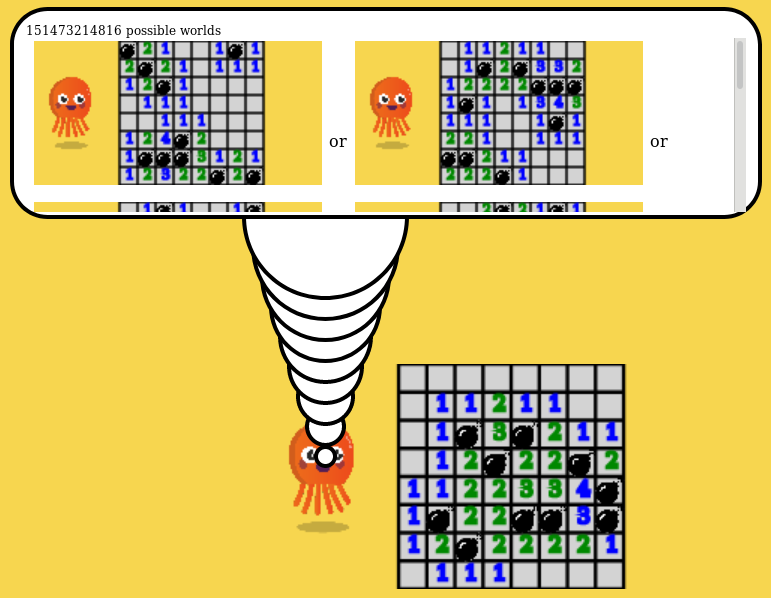
\includegraphics[height=5cm]{images/HW_minesweeper_easy.png}
\end{center}


\begin{example}
	Minesweeper easy $8 \times 8$ with 10 bombs: $> 10^{12}$ possible worlds.
\end{example}
\end{frame}

\begin{frame}
\frametitle{State explosion problem}


%2629575 * 245157 * 6435


\begin{center}
	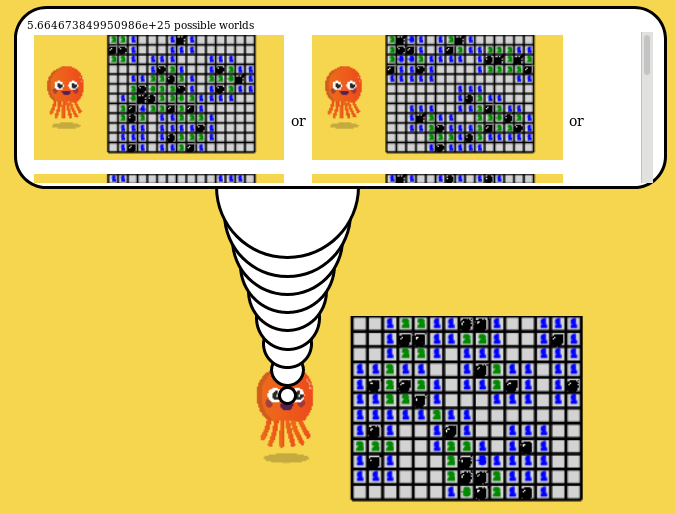
\includegraphics[height=5cm]{images/hintikkas_world_minesweeper.png}
\end{center}


\begin{example}
	Minesweeper $10 \times 12$ with 20 bombs: $> 10^{25}$ possible worlds.
\end{example}
\end{frame}


\begin{frame}
	\frametitle{Belote}
	\begin{center}
		\includegraphics[height=7cm]{images/hintikkas_world_belote.png}
	
	\end{center}

\end{frame}

\subsection{Solution}

\begin{frame}
\frametitle{Solution to the state explosion problem}

\begin{center}
	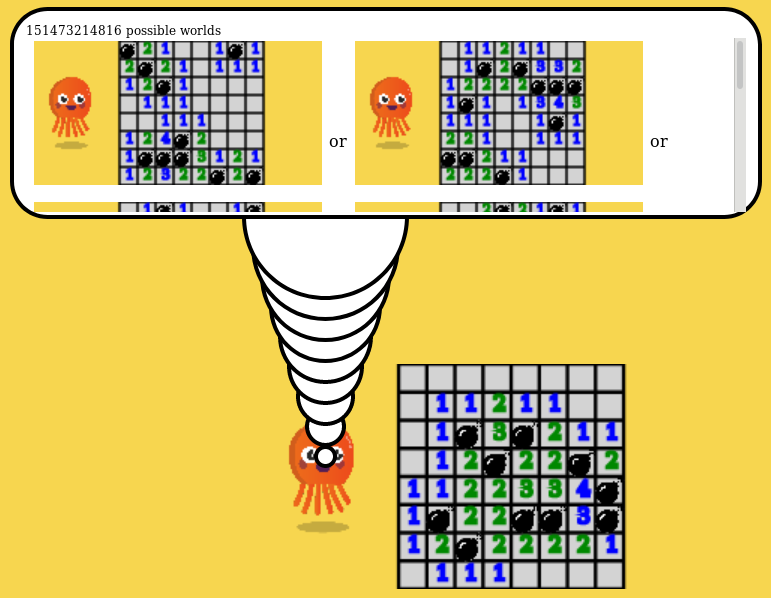
\includegraphics[height=2cm]{images/HW_minesweeper_easy.png}
\end{center}

\vfill
\citeinslide{van Benthem, et al. 2015}, \citeinslide{van Benthem et al. 2018}

\vfill
\begin{block}{ \mycitebiblio{Charrier \_ AAMAS 2017}, \mycitebiblio{Charrier \_ AiML 2018}}
	\begin{itemize}
		\item Succinct representations of epistemic states; {and} actions;
		\item Easy to specify by means of accessibility programs;
		\item Succinct model checking \PSPACE-complete.
	\end{itemize}
\end{block}

\end{frame}



\begin{frame}
	\frametitle{Implementation}

\begin{center}
	\begin{tabular}{lll}
		%Alexandre Niveau & 
		Wrapper of CUDD & C, \texttt{wasm} \\
		 & a library for BDDs & \\[2mm] \hline
		 
		 %Sébastien Gamblin and me & 
		 Succinct epistemic states & Typescript \\
		    and actions  &  \\[2mm]  \hline
		 
		 %Tristan Charrier and me &
		  Examples & Typescript
		 
	\end{tabular}
	\end{center}
	
	
\vfill
\hfill
	\begin{minipage}{7cm}
		\small
	BDD = binary decision diagrams
	
	CUDD = Colorado University Decision Diagram.
	
	wasm = Web Assembly
	\end{minipage}
\end{frame}






